% this file is called up by thesis.tex
% content in this file will be fed into the main document

\chapter{Implementation} % top level followed by section, subsection


% ----------------------- paths to graphics ------------------------

% change according to folder and file names
\ifpdf
    \graphicspath{{7/figures/PNG/}{7/figures/PDF/}{7/figures/}}
\else
    \graphicspath{{7/figures/EPS/}{7/figures/}}
\fi

\section{OpenCSD}

In this section we describe the tools and techniques used with the OpenCSD
framework, detail modules with their respective functionality and show the
external dependencies as well as internal relationships of these modules. 
Followed by, sections on filesystem and offloading implementation details.

\subsection{Framework}

Firstly, OpenCSD consist of many external dependencies, most prominently
\textit{Storage Performance Development Kit} (SPDK) \cite{spdk} and uBPF
\cite{ubpf}. These technolgies are used as userspace NVMe SSD driver and as
virtual machine for the eBPF ISA respectively. Reusing as many as pre-existing
technologies as possible increases the change of familiarity aiding ease of use.
More prominently, these existing technologies dramatically lower the amount of
development effort required to create the prototype. However, our design
requirements demand these dependencies be installed in an isolated way. To do
this OpenCSD configures an isolated build environment with dependencies made
available through an environment file. Moreover, this file configures variables
such as \textit{PATH} and \textit{LD\_LIBRARY\_PATH}. In addition, OpenCSD
offers a QEMU installation and accompanying qcow image to emulate a ZNS SSDs.
This is to overcome the limited availability of these SSDs as stated in the
design requirements. However, the use of QEMU for ZNS SSDs is entirely optional.
Finally, CMake \cite{cmake} is used to orchestrate the installation of
dependencies as well as the compilation of binary targets. Due to limitations it
is advised to rerun CMake after each make command, as this  prevents unnecessary
recompilation of external dependencies \footnotemark[9]. The combination of this
isolated dependencies environment managed through CMake with the ability to use
QEMU for ZNS SSDs emulation is ideal to minimize the complexity as exposed to
users of OpenCSD.

\footnotetext[9]{Due to limitations in the evaluation of file presence
conditions which are not reevaluated when executing the generated makefile.}

As said OpenCSD is comprised of modules using a component architecture.
Additionally, Each module is compiled as a static or shared library to reduce
coupling. This creates an explicit nature of exchanging information between
linked libraries that allows to identify feasibility problems at an early stage.
This is opposed to potentially only identifying such issues when creating a
first hardware prototype. A trivial example of such infeasibilities would be
using shared memory mutexes to synchronize filesystem and CSx kernel behaviour.
Several modules are solely an interface with subsequent modules being one or
more concrete implemenations of these interfaces. These module based interfaces
with loose coupling allow for simplified replacement of technologies.

\subsubsection{Modules}

The overall modules of OpenCSD are shown in figure
\ref{figure:moduledependencies} along with any external or internal
dependencies. In addition, we briefly describe the functionality of each module.
Finally, at the end of this subsection we describe the three most prominent
modules of OpenCSD.

% Diagram with overview of different modules and their used as well as
% relationships. Also show integration of open-source technologies.

\begin{figure}
    \centering
	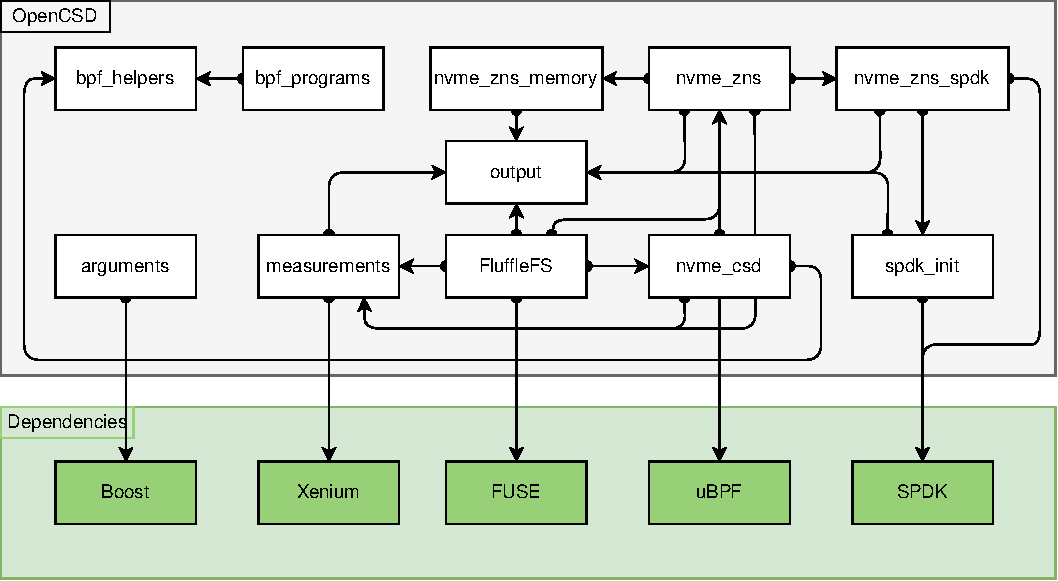
\includegraphics[width=1\textwidth]{resources/images/module-dependencies.pdf}
	\caption{Overview of all OpenCSD components and their depends-on relations}
    % \includesvg[width=0.6\columnwidth]{resources/images/module-dependencies}
    \label{figure:moduledependencies}
\end{figure}

\begin{itemize}
    \item output - Manages stdout and stderr output to the console by
    registering namespaces and providing a variety of log levels.
    \item arguments - Parses command line arguments and splits these into parts
    that can be passed to other modules in a decoupled nature. 
    \item measurements - Low overhead performance instrumentation for functions
    separated by namespaces using high performance lockless unbounded queue
    \cite{Michael1996SimpleFA}.
    \item spdk\_init - Collection of helpers to perform SPDK initialization and
    select ZNS suppporting NVMe namespace.
    \item nvme\_zns - NVMe interface to perform ZNS operations read, write and
    reset. To be used by FluffleFS for decoupled I/O operations.
    \item nvme\_zns\_memory - Memory backed implementation of nvme\_zns
    interface.
    \item nvme\_zns\_spdk - SPDK backed implementation of nvme\_zns interface
    \item nvme\_csd - Simulated extension to the PCIe NVMe protocol that allows
    to perform CSx operations. Execution of kernels is handled through uBPF.
    Utilizes instance of nvme\_zns to perform actual I/O operations performed by
    kernel.
    \item bpf\_helpers - Collection of headers that define the eBPF ABI
    supported for CSx kernels. ABI to be implemented by device vendor
    or in this case nvme\_csd for simulation. The ABI is filesystem agnostic.
    \item bpf\_programs - Collection of eBPF programs linked at runtime for
    previous ZCSD \cite{lukken2021zcsd} prototype.
    \item FluffleFs - FUSE LFS supporting in-memory snapshots to achieve
    multi-user tenancy with concurrent regular and offloaded filesystem access.
    Utilizes, nvme\_zns and nvme\_csd to achieve functionality.
\end{itemize}

Out of these components nvme\_csd, bpf\_helpers and FluffleFS are the most
essential. They simulate the required changes that would realize such an
architecture.

In short nvme\_csd contains functions that should be made part of a new NVMe
command set and namespace \cite{nvme-command} similar to how ZNS was introduced.
Currently, the functions are overly simplified so there is no use of the actual
command layout as well as lack of queue submissions and completion commands. We
feel the concepts of implementing these are well understood and would not
contribute to the scientific value of this work while introducing substantial
additional complexity.

bpf\_helpers contains the ABI exposed to the eBPF kernels. An ABI is different
from an API in that the functions it defines cannot be found in segments of
code, either included statically or through a shared library. Instead it uses
an ISA specific instruction that can be called with a set of arguments, the
arguments matching the function signature. Alternatively, should the ISA not
have a specific \textit{call} instruction, interrupt requests can be used to
achieve the same functionality. Upon calling the control flow is returned to
the operating system or in our case uBPF where the functions behavior is
implemented. The result is that an ABI allows to define functionality with
vendor agnostic implementations, similar to POSIX for operating systems. It
should be noted that ISAs typically have a hard limit on the number of arguments
that can be supported, in the case of eBPF this is five arguments. Lastly, is
FluffleFS which is described in the next section in detail.

Out of all modules only nvme\_zns has been given an abstract interface so the
underlying technologies can be easily replaced. However, we argue the design
requirements are still met as there are virtually no replacements for
technologies used in other modules such as uBPF and FUSE\footnotemark[10].
In addition, we feel it would have beneign benefits to create abstract
interfaces of the C++ STL. Our solution allows for replacing technologies with
readily available alternatives without creating unnecessary interfaces.

\footnotetext[10]{While alternative technolgies to implement filesystems exist
none of them are in userspace. As a result we argue there is no alternative to
FUSE.}

\subsection{Filesystem}

% Two write pointers, one for RANDOM ZONE and one for LOG ZONE. Use of ZNS is
% optional but allows for lower write-amplification and more explicit garbage
% collection

\subsubsection{Concurrency}

\subsection{Offloading}

% Filesystem extended attributes, PID + INODE

\section{Iterations}

This section is covered separetely to prevent clutter in the overall design and
implementation sections. This process consisted of four destinct iterations.
Two relating primarily to the framework, one to the filesystem and one to
offloading. This section describes each iteration briefly before going in more
detail. Firstly regarding framework iterations we see the distinct decision
to switch from a multi process architecture using mmap for shared memory maps to
a monolithic application. The second iteration lead to switching away from the
design of an accelerator API, much like Vulkan \cite{vulkan} or OpenCL, to an
artificial extension of the NVMe namespace. The third iteration changed the use
rtld\_next \cite{rtldnext} to using a practical filesystem with FUSE. Lastly, as
computational storage API our work switched from using
\textit{Portable Operating System Interface} (POSIX) fadvise \cite{fadvise} to
extended attributes.

For each of these four iterations the advantages of the change as well as the
major issues with the previous solution are described. Each iteration is
described in the same order as previously defined.

\subsection{Shared Memory Monolith}

Modern operating systems offer fastly different methods to write sofware. From
kernel modules, to distributed processes, UNIX pipes and shared memory maps.
Choosing the right model impacts practicalities such as the amount of
development effort required and the robustness of the final solution. 
Furtermore, depending on the software architecture some solutions will be better
suited than others.

During the design the use of shared memory maps was replaced with using regular
shared memory. While both solutions provide shared memory they are fundamentally
different. A shared memory map is a file, leveraging the well known UNIX
principle \textit{everything is a file}, that allows two or more processes to
share a region of memory. While regular shared memory is limited to a single
process although it could share this memory with additional threads.

this single process shared memory solution is one of the most common found in
software today. The concepts of such a program are very well understood as
well as the development using imperative languages being straightforward.

While shared memory maps are typically found in device drivers, such as those
for graphics cards, their use consistutes severe additional development effort.
In conjuction with our design being a simulation there is no scientific value in
using shared memory maps for our design.

\subsection{NVMe Namespace Command Set}

\subsection{FUSE Filesystem}

\subsection{Extended Attributes}

% ---------------------------------------------------------------------------
% ----------------------- end of thesis sub-document ------------------------
% ---------------------------------------------------------------------------